\documentclass[tikz, border=2pt]{standalone}
% main document, called main.tex
\usepackage{tikz}
\usetikzlibrary{bayesnet}

\begin{document}

% \title{shift-one-source-gen}
% \author{Dhruv Patel}
% \date{July 2022}

\tikzstyle{emptynode} = [rectangle, draw=black!0, minimum size=5mm]
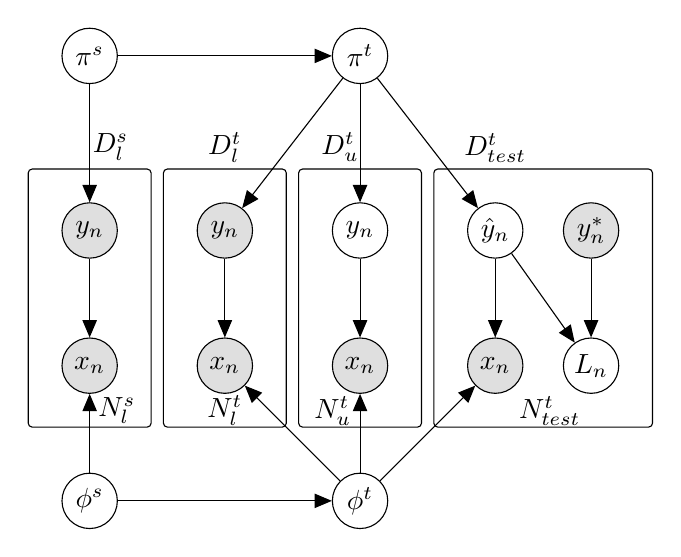
\begin{tikzpicture}
	\node[latent]  (ws) {$\pi^s$};
	\node[obs, below = 15mm of ws](y1n){$y_n$};
	\node[obs, below = of y1n](x1n){$x_n$};
	\node[obs, right=  of y1n](y2n){$y_n$};
	\node[obs, below= of y2n](x2n){$x_n$};
	\node[latent, right = of y2n](y3n){$y_n$};
	\node[latent, above =  15mm of y3n](wt){$\pi^t$};
	\node[obs, below= of y3n](x3n){$x_n$};
	\node[latent, right = of y3n](yhat){$\hat y_n$};
	\node[obs, right = 5mm of yhat](ystar){$y^*_n$};
	\node[obs, below= of yhat](x4n){$x_n$};
	\node[latent, below= of ystar](ln){$L_n$};
	\node[latent, below = of x1n](psis){$\phi^s$};
	\node[latent, below = of x3n](psit){$\phi^t$};
	\node[draw=black,thin,fit=(y1n)(x1n), rounded corners=.05cm,inner sep=12pt](rect1)  {};
	\node[draw=black,thin,fit=(y2n)(x2n), rounded corners=.05cm,inner sep=12pt](rect2)  {};
	\node[draw=black,thin,fit=(y3n)(x3n), rounded corners=.05cm,inner sep=12pt](rect3)  {};
	\node[draw=black,thin,fit=(yhat)(ystar)(x4n)(ln), rounded corners=.05cm,inner sep=12pt](rect4)  {};
	\edge{ws}{wt};
	\edge{ws}{y1n};
	\edge{wt}{y2n, y3n, yhat};
	\edge{y1n}{x1n};
	\edge{y2n}{x2n};
	\edge{y3n}{x3n};
	\edge{yhat}{x4n};
	\edge{yhat,ystar}{ln};
	\edge{psis}{x1n};
	\edge{psit}{x2n, x3n, x4n};
	\node[const, above  = 0.5cm of y2n](c1){$D^t_l$};
	\node[const, left = 1cm of c1]{$D^s_l$};
	\node[const, right = 1cm of c1]{$D^t_u$};
	\node[const, above  = 0.5cm of yhat]{$D^t_{test}$};
	\node[const, below =2.95cm of c1](cbelow){$N^t_l$};
	\node[const, left = 0.9cm of cbelow]{$N^s_l$};
	\node[const, right = 0.9cm of cbelow]{$N^t_u$};
	\node[const, right = 3.5cm of cbelow]{$N^t_{test}$};
	\edge{psis}{psit};
	
\end{tikzpicture}
\end{document}
